\documentclass[]{article}
\usepackage[T1]{fontenc}
\usepackage{lmodern}
\usepackage{amssymb,amsmath}
\usepackage{ifxetex,ifluatex}
\usepackage{fixltx2e} % provides \textsubscript
% use upquote if available, for straight quotes in verbatim environments
\usepackage{graphicx}
\usepackage{float}
 \usepackage[margin=0.5cm]{geometry} 

\title{Explanation of Dispersion}
\author{Han Zhang}
\date{March 12, 2015}

\begin{document}
\maketitle

\begin{figure}[ht]
\begin{minipage}[b]{0.5\linewidth}
\centering
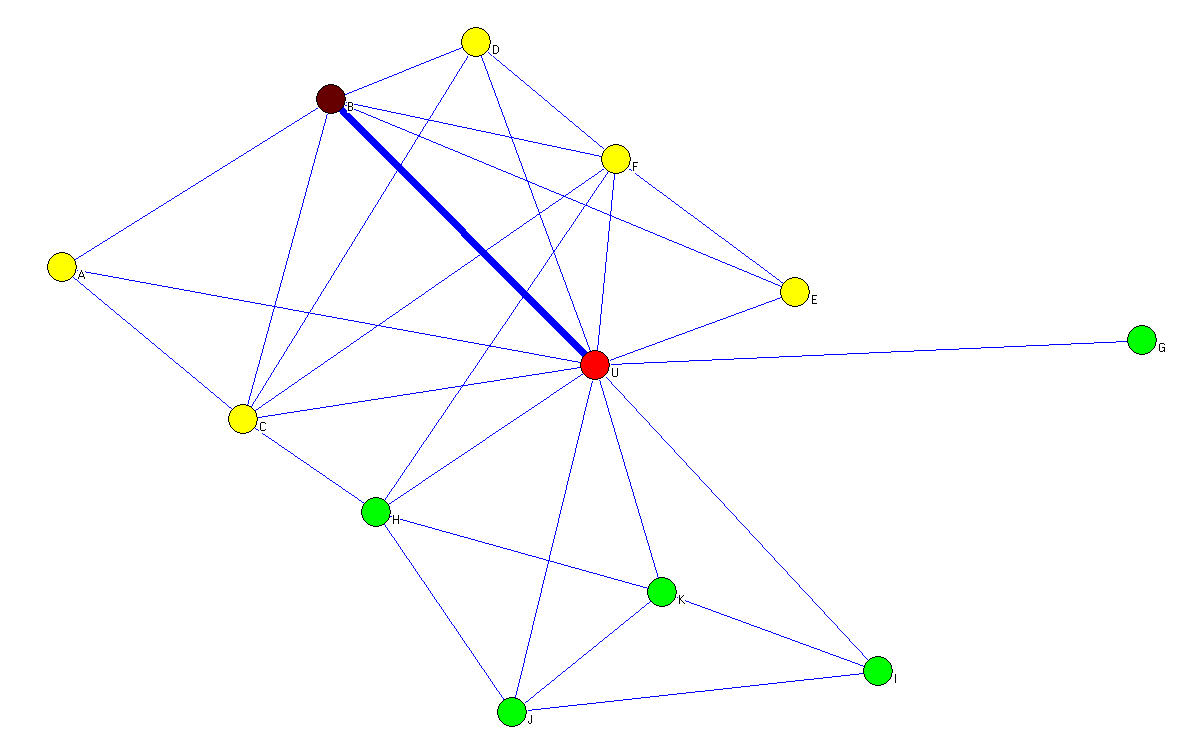
\includegraphics[width=\textwidth]{1.jpg}
\caption{($U,B$) as predicted partner. Yellow nodes are common friends of ($U,B$).}
\label{fig:figure1}
\end{minipage}
\hspace{0.5cm}
\begin{minipage}[b]{0.5\linewidth}
\centering
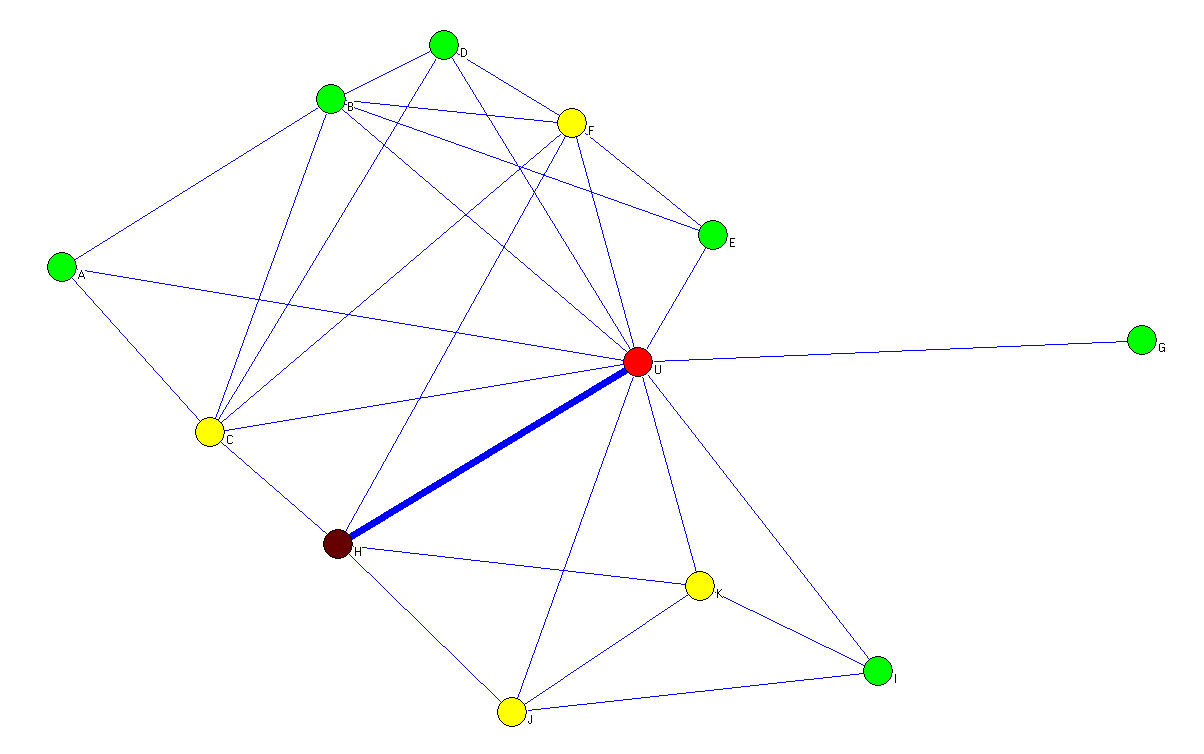
\includegraphics[width=\textwidth]{2.jpg}
\caption{($U,H$) as predicted partner. Yellow nodes are common friends of ($U,H$)}
\label{fig:figure2}
\end{minipage}
\end{figure}

This note illustrate the concept of \textbf{dispersion}--a new way of measuring tie strength--as defined in Backstrom and Kleinberg, "Romantic Partnerships and the Dispersion of Social Ties: A Network Analysis of Relationship Status on Facebook".

Their motivation is: given a person $U$, they want to find whether an friend
of $U$ is his/her romantic partner. 
This is a real business task in Facebook.
We can predict whether $U$ and a
friend $V$ is romantic partner based on \textbf{embeddedness}, defined as the
number of common friends between $U$ and $V$. 
Embeddedness is the traditional way of measuring tie strength.
For instance, compare Fig. 1 and 2, we wish to know who is possible partner of $U$:

\begin{itemize}
\itemsep1pt\parskip0pt\parsep0pt
\item
  in Fig. 1, embeddedness between $U$ and $B$ is 5 (yellow nodes
  are common friends)
\item
  in Fig. 2, embeddedness between $U$ and $H$ is 4 (yellow
  nodes are common friends)
\end{itemize}

We will think that $U$ and $B$ will be more likely to be partner than
with $H$ based on embeddedness.
 But it may not necessarily be true: 
 $U$ and $B$ are in the same foci,
which makes them have more common friends. So Backstrom and Kleinberg
invented the idea of dispersion.


\begin{figure}[ht]
\begin{minipage}[b]{0.5\linewidth}
\centering
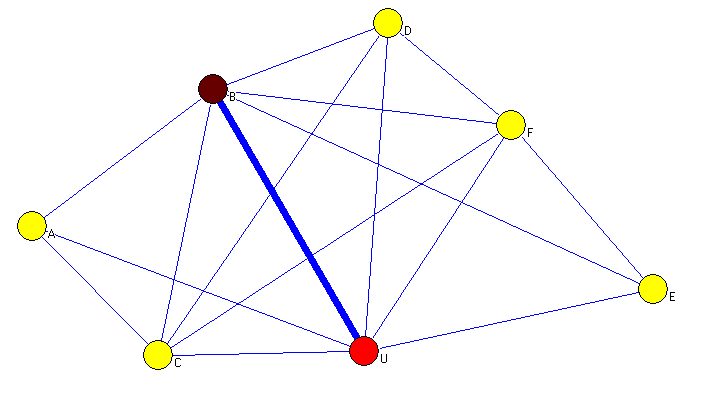
\includegraphics[width=\textwidth]{p1dispersion.png}
\caption{($U,B$) as predicted partner. Only common friends of ($U,B$) are shown.}
\label{fig:figure1}
\end{minipage}
\hspace{0.5cm}
\begin{minipage}[b]{0.5\linewidth}
\centering
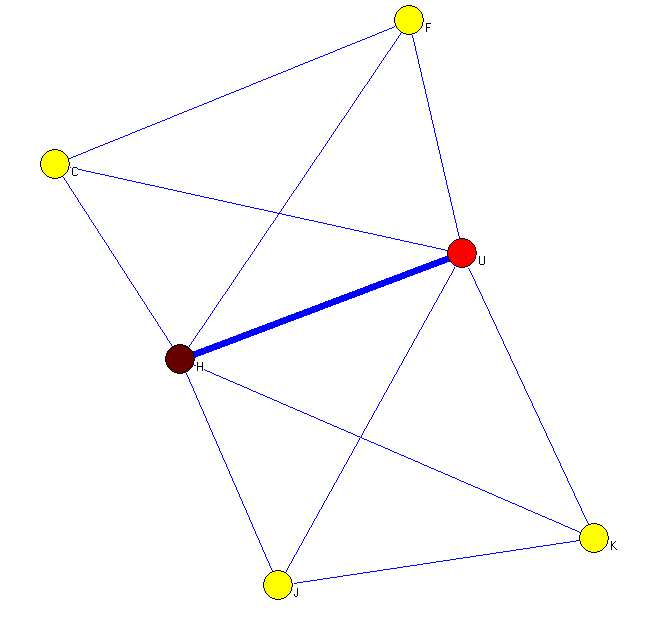
\includegraphics[width=\textwidth]{p2dispersion.png}
\caption{($U,H$) as predicted partner.  Only common friends of ($U,H$) are shown.}
\label{fig:figure2}
\end{minipage}
\end{figure}


Dispersion, $disp(U,V)$ is defined as following:
 the set of all common friends of $U$ and $V$ is
$C_{UV}$. (yellow nodes in the image!) Then, for each pair of node $s,t$
in common neighbors set $C_{UV}$
\[disp(U,V) = \sum_{s,t \in C_{UV}} d_{st}\]

$d_{st}$ = 1, if there is

\begin{enumerate}
\item
  No direct link betwen $s$ and $t$
\item
  No other common friends which is also $U$'s friend
\end{enumerate}

or otherwise $d_{st}=0$, which suggest that $s,t$ may belong to the same
foci and are not ``dispersed''.
The larger the dispersion between two nodes, the stronger their tie is. 

Use the same network, we predict who is the partner of $U$ based on dispersion:
\begin{itemize}
\itemsep1pt\parskip0pt\parsep0pt
\item
  In Fig. 3, $disp(U,B)$=1: there is only one pair whose $d$ is
  1: $(A,E)$.
\item
  In Fig. 3, $disp(U,H)$=4: there are four pairs whose $d$ is 1:
  $(F,K)$,$(F,J)$,$(C,J)$,$(C,K)$.


  \begin{itemize}
  \itemsep1pt\parskip0pt\parsep0pt
  \item
    all other pairs, such as $(A,D)$ have common friend $C$ who is also
    $U$'s friend; $(F,E)$ are directly linked.
  \end{itemize}
\end{itemize}
Base on dispersion we will predict that $U,H$ are more likely to be romantic partners since their tie strength is stronger.

\textbf{Now, exercise:}

See Fig. 5 and 6. What is the number of embeddedess, and dispersion
for $(U,C)$, and $(U,A)$ link ? Do you think whether those two are more likely to
be a romantic relationship, comparing with $(U,H)$?


\begin{figure}[!htbp]
\begin{minipage}[b]{0.5\linewidth}
\centering
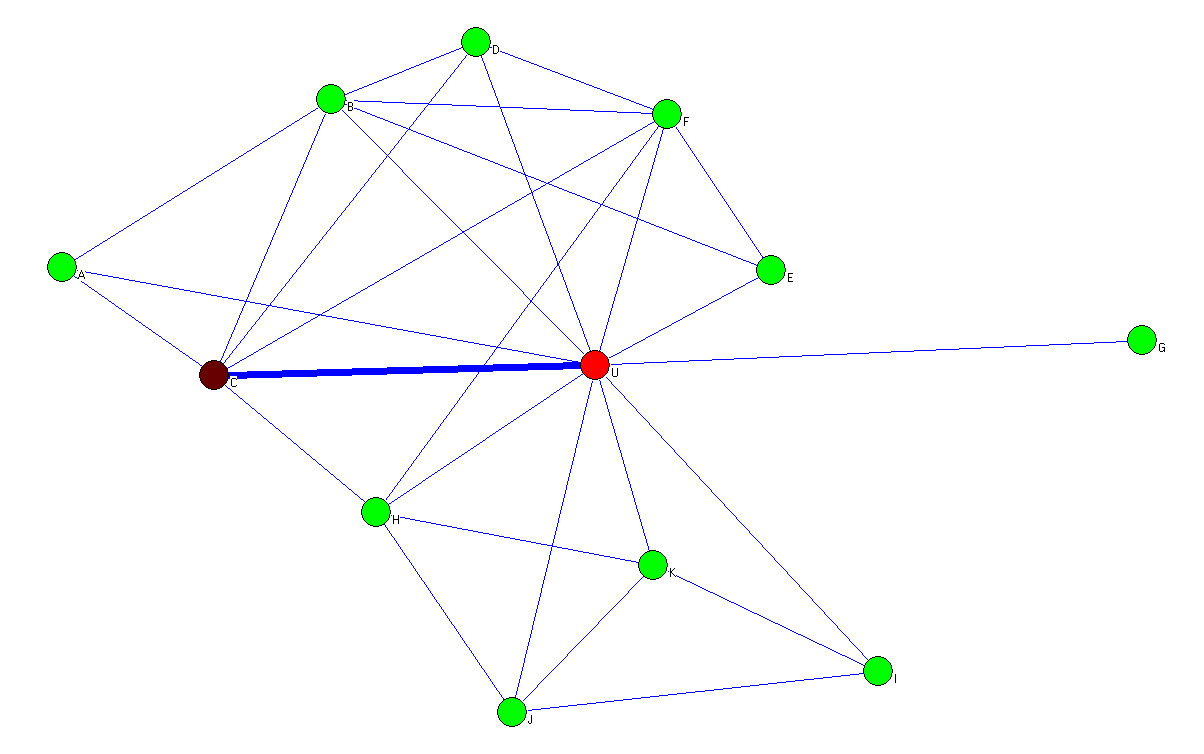
\includegraphics[width=\textwidth]{exp_embeddedness.jpg}
\caption{($U,C$) as predicted partner}
\label{fig:figure1}
\end{minipage}
\hspace{0.5cm}
\begin{minipage}[b]{0.5\linewidth}
\centering
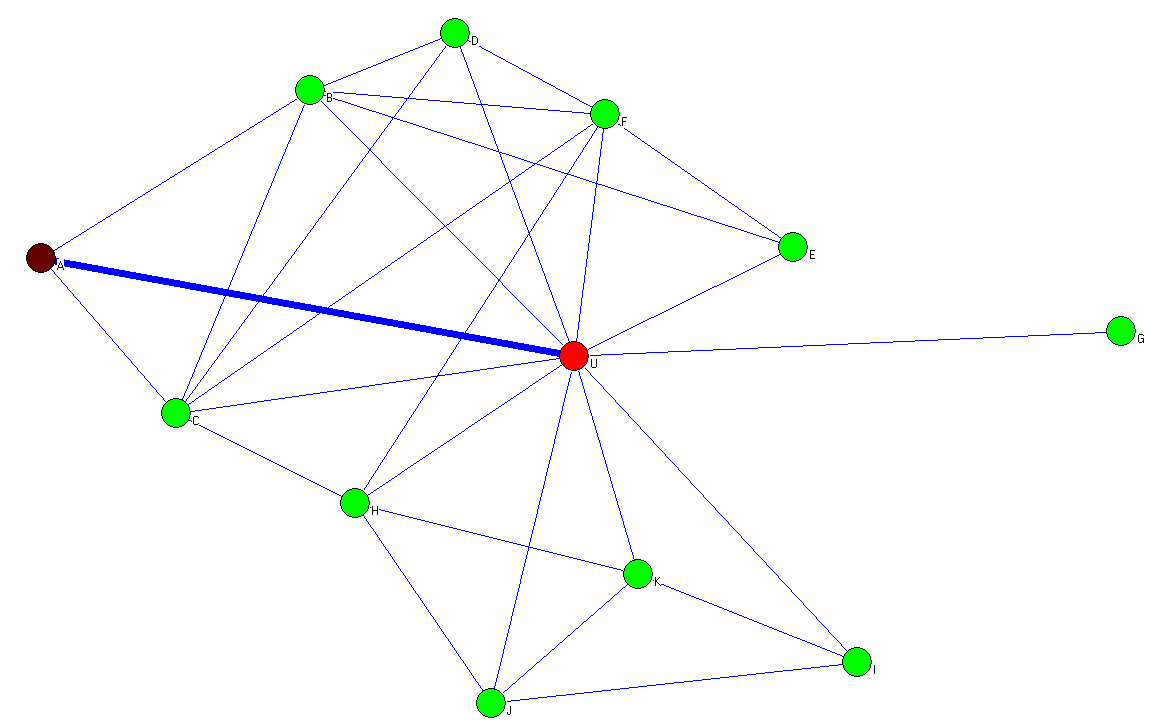
\includegraphics[width=\textwidth]{p6embedd.png}
\caption{($U,A$) as predicted partner. }
\label{fig:figure2}
\end{minipage}
\end{figure}


\newpage

Tips: it is easy to calculate embeddedness.
For dispersion, extract a similar subgraph which only contained common neighbors of the tie we wish to predict, as the following.
See Fig. 7 and 8 for examples, but you may let students to do it.

\begin{figure}[!htbp]
\begin{minipage}[b]{0.5\linewidth}
\centering
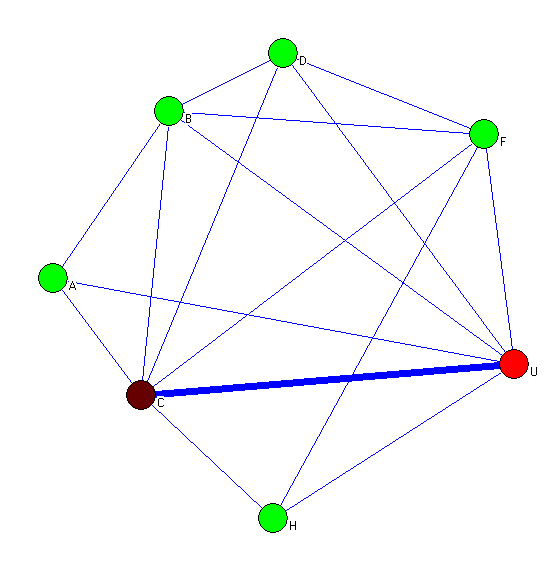
\includegraphics[width=\textwidth]{exp_dispersion.png}
\caption{($U,C$) as predicted partner}
\label{fig:figure1}
\end{minipage}
\hspace{0.5cm}
\begin{minipage}[b]{0.5\linewidth}
\centering
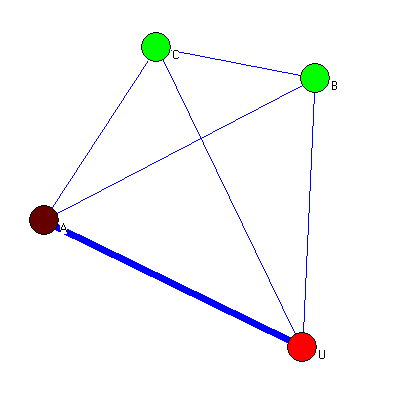
\includegraphics[width=\textwidth]{p6disper.png}
\caption{($U,A$) as predicted partner. }
\label{fig:figure2}
\end{minipage}
\end{figure}



\end{document}
